\documentclass[a4paper,12pt]{article}

% =============================================================================
% Cấu hình tiếng Việt và trình bày
% =============================================================================
\usepackage[utf8]{inputenc}
\usepackage[T5]{fontenc}
\usepackage[vietnamese]{babel}
\shorthandoff{"}
\usepackage{geometry}
\geometry{top=2.2cm,bottom=2.2cm,left=2.4cm,right=2.2cm}
\usepackage{enumitem}
\usepackage{amsmath,amssymb}
\usepackage{graphicx}
\usepackage{subcaption}
\usepackage{float}
\usepackage{booktabs}
\usepackage{tabularx}
\usepackage{longtable}
\usepackage{array}
\usepackage{xcolor}
\usepackage{listings}
\usepackage{tikz}
\usetikzlibrary{arrows.meta,positioning,shapes.geometric,fit,calc}
\usepackage{xurl}
\usepackage{hyperref}
\hypersetup{
  colorlinks=true,
  linkcolor=black,
  urlcolor=blue,
  citecolor=black
}
\usepackage{fancyhdr}
\usepackage{caption}

\definecolor{codegreen}{rgb}{0,0.45,0}
\definecolor{codegray}{rgb}{0.45,0.45,0.45}
\definecolor{codepurple}{rgb}{0.55,0,0.75}
\definecolor{backcolour}{rgb}{0.96,0.96,0.94}
\definecolor{uetblue}{RGB}{0,78,135}
\definecolor{softblue}{RGB}{226,240,252}
\definecolor{softgreen}{RGB}{227,245,232}
\definecolor{softorange}{RGB}{255,239,216}

\lstdefinestyle{mystyle}{
  backgroundcolor=\color{backcolour},
  commentstyle=\color{codegreen}\itshape,
  keywordstyle=\color{magenta}\bfseries,
  numberstyle=\tiny\color{codegray},
  stringstyle=\color{codepurple},
  basicstyle=\ttfamily\footnotesize,
  breaklines=true,
  keepspaces=true,
  numbers=left,
  numbersep=6pt,
  showspaces=false,
  showstringspaces=false,
  tabsize=2,
  frame=single,
  rulecolor=\color{black},
  columns=fullflexible
}
\lstset{style=mystyle}
\renewcommand{\lstlistlistingname}{Danh mục đoạn mã}
\renewcommand{\lstlistingname}{Đoạn mã}

\setlength{\parskip}{2.2mm}
\setlength{\parindent}{0.8cm}
\renewcommand{\arraystretch}{1.18}
\pagestyle{fancy}
\fancyhf{}
\lhead{\small\textit{Tương tác Người -- Robot}}
\rhead{\small Báo cáo bài tập thực hành 03}
\cfoot{\thepage}
\renewcommand{\headrulewidth}{0.5pt}

\newcommand{\code}[1]{\texttt{#1}}
\newcommand{\skill}[1]{\texttt{#1}}

\begin{document}

% =============================================================================
% Trang bìa
% =============================================================================
\begin{titlepage}
\begin{tikzpicture}[remember picture,overlay]
  \draw[line width=3pt,uetblue]
    ([xshift=1.8cm,yshift=-1.8cm]current page.north west) rectangle
    ([xshift=-1.8cm,yshift=1.8cm]current page.south east);
\end{tikzpicture}
\begin{center}
  \vspace*{-1cm}
  {\scshape\Large ĐẠI HỌC QUỐC GIA HÀ NỘI\\
  TRƯỜNG ĐẠI HỌC CÔNG NGHỆ}\[0.5cm]

  \IfFileExists{images/logo_uet.png}{
    
\includegraphics[width=3.3cm]{images/logo_uet.png}\\[0.45cm]
  }{
    {\Large\bfseries VNU--UET}\\[0.7cm]
  }

  {\scshape\large\bfseries BÁO CÁO THỰC HÀNH MÔN HỌC}\\[0.25cm]
  {\scshape\Large\bfseries TƯƠNG TÁC NGƯỜI -- ROBOT}\\[0.65cm]
  {\scshape\LARGE\bfseries BÀI THỰC HÀNH 03}\\[0.35cm]
  {\Large\bfseries LLM SKILL PLANNING VỚI GRIPPER VÀ CAMERA}\\[0.75cm]

  \begin{tabular}{ll}
    \textbf{Giảng viên hướng dẫn:} & PGS. TS. Hoàng Văn Xiêm \\
                                   & KS. Nguyễn Quốc Bảo \\[0.45cm]
    \textbf{Sinh viên thực hiện:}  & Lê Anh Tuấn Bằng \\
    \textbf{Mã số sinh viên:}      & 23020723 \\
    \textbf{Nhánh mã nguồn:}       & \code{assignments\_3} \\
    \textbf{Package chính:}        & \code{ur3\_llm\_control}
  \end{tabular}

  \vfill
  \textbf{Hà Nội, 2026}
\end{center}
\end{titlepage}

\pagenumbering{roman}
\tableofcontents
\newpage
\listoffigures
\listoftables
\lstlistoflistings
\newpage
\pagenumbering{arabic}

% =============================================================================
\section{Tổng quan bài toán}

\subsection{Mục tiêu của Bài thực hành 03}
Bài thực hành 03 phát triển hệ thống Bài 02 từ mức lập kế hoạch kỹ năng trong
môi trường biết trước thành một hệ thống thao tác có phản hồi môi trường. Robot
UR3 nhận câu lệnh tự nhiên, dùng LLM để hiểu ý định và lựa chọn kỹ năng, nhưng
phải quan sát bàn bằng camera trước khi thực hiện. Hệ thống cần gắp, giữ, mang và
thả vật bằng gripper thật trong Gazebo; không được thay đổi trực tiếp pose của
khối để giả lập thao tác.

Không gian làm việc gồm một UR3, một gripper hai ngón, một camera RGB cố định
phía trên, một bàn, năm khối màu và ba vùng đích. Vì số khối lớn hơn số vùng
đích, một vùng được yêu cầu có thể đang bị vật khác chiếm. Robot phải phát hiện
xung đột, chọn vị trí tạm, dời vật cản rồi mới hoàn thành yêu cầu chính.

\subsection{Các yêu cầu bắt buộc và cách đáp ứng}
\begin{longtable}{p{0.27\textwidth}p{0.66\textwidth}}
\caption{Đối chiếu yêu cầu đề bài với hiện thực hệ thống}\label{tab:requirements}\\
\toprule
\textbf{Yêu cầu} & \textbf{Cách hiện thực trong dự án}\\
\midrule
\endfirsthead
\toprule
\textbf{Yêu cầu} & \textbf{Cách hiện thực trong dự án}\\
\midrule
\endhead
UR3/UR3e và MoveIt 2 & UR3 được nạp qua driver mô phỏng, MoveIt 2 lập kế hoạch
cho planning group \code{ur\_manipulator}; KDL giải IK và OMPL xử lý các đoạn
di chuyển tự do có kiểm tra va chạm.\\
Gripper vật lý & Hai ngón kẹp là hai khớp tịnh tiến có controller vị trí,
collision pad, ma sát và contact sensor trong Gazebo. Vật chỉ được attach sau
khi hình học và tiếp xúc đã được xác nhận.\\
Camera bắt buộc & Camera RGB trên cao phát ảnh 640$\times$480 tại 5 Hz. Node
OpenCV phân đoạn HSV, tính tâm contour, đổi pixel sang tọa độ bàn và công bố
trạng thái các zone.\\
Năm block, ba zone & Có \code{red}, \code{yellow}, \code{blue}, \code{green},
\code{purple}; ba vùng đích A/B/C và ba vùng đệm tạm.\\
Xử lý vùng bị chiếm & \code{prepare\_plan()} đọc \code{zone\_occupants}, chọn
vùng đệm trống và chèn cặp \skill{pick/place} dời vật cản trước hành động chính.\\
LLM không sinh quỹ đạo & LLM chỉ trả JSON gồm tên skill và tham số. Validator
chặn tên lạ, tham số sai và chuỗi thao tác không hợp lệ; MoveIt 2 mới sinh quỹ
đạo khớp.\\
Kiểm tra trước và sau & Camera phải sẵn sàng trước khi nhận lệnh; kế hoạch được
mô phỏng logic trước khi chạy; sau khi hoàn thành camera xác nhận các vị trí
đích.\\
\bottomrule
\end{longtable}

\subsection{Cá nhân hóa theo mã số sinh viên}
Với MSSV \code{23020723}, hai chữ số cuối là $XX=23$:
\begin{equation}
P = XX \bmod 6 = 23 \bmod 6 = 5.
\end{equation}
Theo quy ước $P=5$, ánh xạ bắt buộc là:
\begin{center}
\begin{tabular}{ccc}
\toprule
\textbf{Zone A} & \textbf{Zone B} & \textbf{Zone C}\\
\midrule
\code{blue\_cube} & \code{yellow\_cube} & \code{red\_cube}\\
\bottomrule
\end{tabular}
\end{center}
Ánh xạ được tính từ \code{student\_config.yaml}. Đối với lệnh sắp xếp theo
MSSV, LLM nhận diện ý định nhưng không được tự chọn hoán vị màu. Module
\code{student\_utils.py} sinh kế hoạch xác định từ trạng thái camera, giữ thứ tự
A--B--C và một lớp hậu kiểm mô phỏng toàn bộ các lệnh \skill{place} để bảo đảm
kết quả cuối đúng ánh xạ trên trước khi robot chuyển động.

% =============================================================================
\section{Kiến trúc hệ thống}

\subsection{Kiến trúc phân tầng}
Hệ thống duy trì ranh giới rõ giữa suy luận cấp cao và điều khiển chuyển động.
Hình~\ref{fig:architecture} mô tả luồng dữ liệu chính.

\begin{figure}[H]
\centering
\begin{tikzpicture}[
  node distance=6mm,
  block/.style={draw,rounded corners,align=center,minimum width=8.2cm,
    minimum height=8mm,font=\small},
  arrow/.style={-{Latex[length=2.2mm]},thick}
]
\node[block,fill=softblue] (user) {Câu lệnh tự nhiên: tiếng Việt hoặc tiếng Anh};
\node[block,fill=softblue,below=of user] (llm) {LLM Planner qua 9Router\\chọn skill, tham số và thứ tự};
\node[block,fill=softorange,below=of llm] (safety) {Plan Safety + Task Validator\\đối chiếu camera, giải phóng zone, kiểm tra whitelist};
\node[block,fill=softgreen,below=of safety] (executor) {Skill Executor + Robot Skills\\\skill{pick}, \skill{place}, \skill{swap}, \skill{home}, \ldots};
\node[block,fill=softgreen,below=of executor] (moveit) {MoveIt 2: IK, Cartesian Path, OMPL, PlanningScene};
\node[block,fill=softblue,below=of moveit] (robot) {UR3 + gripper hai ngón + vật lý Ignition Gazebo};
\node[block,fill=softorange,right=13mm of safety,minimum width=4.3cm] (camera) {Camera + OpenCV\\vị trí cube, zone trống/bận};
\draw[arrow] (user)--(llm);
\draw[arrow] (llm)--(safety);
\draw[arrow] (safety)--(executor);
\draw[arrow] (executor)--(moveit);
\draw[arrow] (moveit)--(robot);
\draw[arrow] (camera.west)--(safety.east);
\draw[arrow] (robot.east) -| (camera.south);
\end{tikzpicture}
\caption{Kiến trúc điều khiển phân tầng của Bài thực hành 03}
\label{fig:architecture}
\end{figure}

\subsection{Các node, module và giao tiếp chính}
\begin{table}[H]
\centering
\caption{Vai trò của các thành phần phần mềm}
\label{tab:modules}
\begin{tabularx}{\textwidth}{p{0.29\textwidth}X}
\toprule
\textbf{Thành phần} & \textbf{Vai trò}\\
\midrule
\code{llm\_interactive\_node} & Điều phối toàn chu trình, khóa chống nhận hai
lệnh đồng thời, lấy scene state, gọi planner, validator và executor.\\
\code{llm\_planner.py} & Gửi prompt kèm trạng thái camera tới 9Router, chuẩn
hóa JSON/function call, xử lý tiếng Việt và ràng buộc ánh xạ MSSV.\\
\code{plan\_safety.py} & Chuẩn hóa tên zone, dời vật cản, chọn buffer và tối
ưu thứ tự các cặp thao tác độc lập.\\
\code{task\_validator.py} & Whitelist skill/object/zone và mô phỏng trạng thái
tay kẹp để kiểm tra tiền điều kiện của từng bước.\\
\code{skill\_executor.py} & Thực thi tuần tự, dừng ngay tại lỗi, bỏ qua thao tác
thừa nếu vật đã ở đích và yêu cầu camera xác nhận kết quả cuối.\\
\code{robot\_skills.py} & Hiện thực chuyển động, gripper, contact, attach/detach,
PlanningScene và các skill nâng cao.\\
\code{camera\_perception.py} & Xử lý ảnh HSV, đổi pixel--world, phân loại vị trí,
phát ảnh annotated và scene state JSON.\\
\code{scene\_spawner.py} & Phát marker RViz, TF, bàn, khay và nhãn trực quan.\\
\bottomrule
\end{tabularx}
\end{table}

Các topic/service/action quan trọng gồm \code{/camera/image\_raw},
\code{/camera/camera\_info}, \code{/scene/camera\_state},
\code{/camera/image\_annotated}, \code{/gripper/left\_contacts},
\code{/gripper/right\_contacts}, \code{/move\_action},
\code{/compute\_cartesian\_path}, \code{/execute\_trajectory} và
\code{/apply\_planning\_scene}.

\subsection{Môi trường Gazebo và RViz}
Mặt bàn có cao độ làm việc $z=0$. Năm cube có kích thước
$40\times40\times40$ mm, đặt trên năm khay nguồn tại $x=0.24$ m. Ba vùng đích
nằm trên hàng $x=0.35$ m; các zone tạm nằm ở biên hai phía và tại
$(0.45,0.00)$ m. Màu nền vùng đích trong Gazebo và RViz tuân theo $P=5$: A
xanh lam, B vàng, C đỏ. Màu khay dùng độ bão hòa thấp để bộ lọc HSV không nhầm
khay với cube.

\begin{figure}[H]
\centering
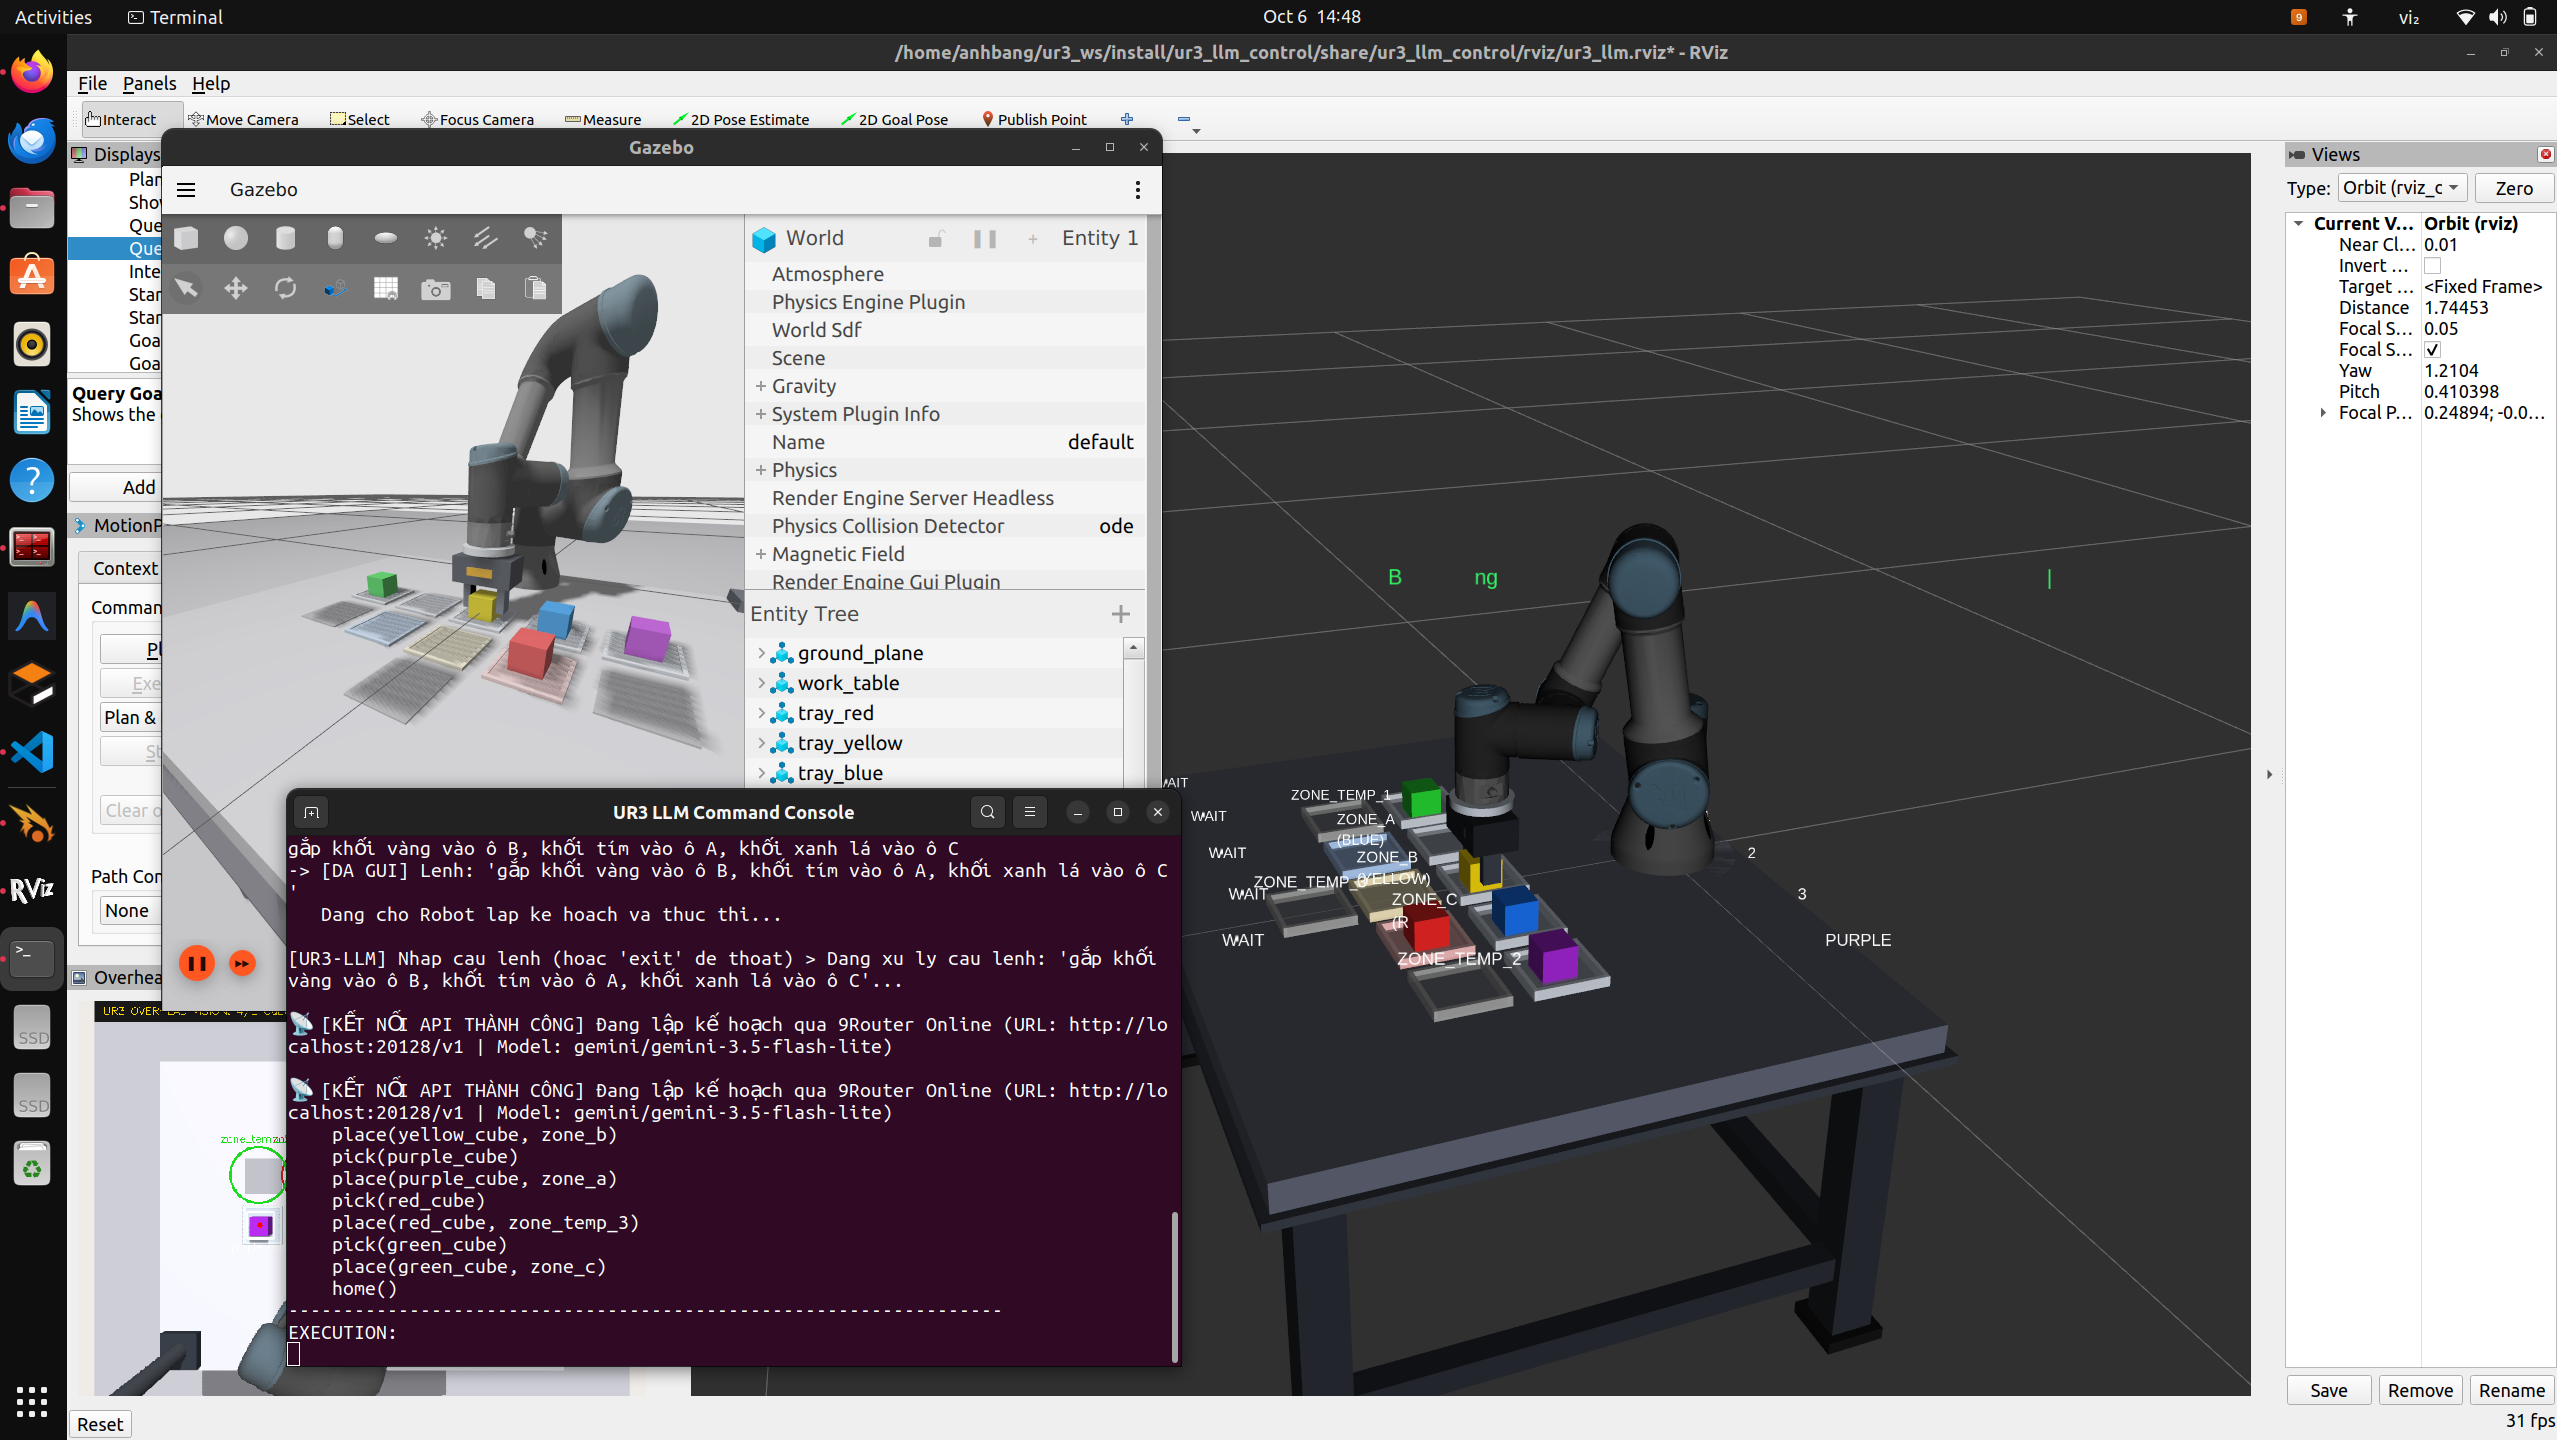
\includegraphics[width=0.98\textwidth]{images/system_overview.png}
\caption{Toàn cảnh hệ thống: Gazebo, RViz, ảnh camera và console LLM}
\label{fig:system-overview}
\end{figure}

Physics chạy bước $2$ ms (500 Hz), phù hợp với controller. PlanningScene chứa
bàn và các cube không được gắp; cube đang cầm được chuyển từ world collision
object sang attached collision object để MoveIt xét kích thước vật trong quá
trình mang.

% =============================================================================
\section{Camera và nhận thức trạng thái môi trường}

\subsection{Lựa chọn camera cố định trên cao}
Camera đặt tại $(0.30,0.00,0.92)$ m và nhìn vuông góc xuống bàn. Với FOV ngang
$1.15$ rad, camera nhìn đồng thời năm khay nguồn, ba zone đích và ba vị trí tạm.
Cách bố trí này phù hợp với yêu cầu lập kế hoạch toàn cục: robot biết zone nào
đang bận trước khi bắt đầu, đồng thời có thể chọn buffer mà không phải di chuyển
cánh tay để quan sát từng nơi.

Camera gắn trên cổ tay hữu ích cho căn chỉnh cục bộ, nhưng vùng nhìn thay đổi
theo robot, dễ bị chính gripper che và cần hiệu chuẩn hand--eye. Bài toán này ưu
tiên trạng thái toàn bàn nên dùng camera cố định. Trong một hệ thống thật có thể
bổ sung camera cổ tay cho bước servo thị giác cuối, trong khi camera trên cao
vẫn chịu trách nhiệm lập kế hoạch toàn cục.

\subsection{Chuỗi xử lý ảnh}
Mỗi 0.5 s, node nhận frame mới, chuyển BGR sang HSV và tạo mask riêng cho năm
màu. Màu đỏ dùng hai khoảng hue vì nằm ở hai đầu vòng màu HSV. Phép mở và đóng
hình thái với kernel $5\times5$ loại nhiễu và nối vùng màu bị đứt. Contour hợp
lệ phải có diện tích từ 250 đến 1200 pixel$^2$; giới hạn trên giúp loại phần
khay màu có diện tích lớn hơn cube.

Với contour lớn nhất, tâm ảnh được tính từ moment:
\begin{equation}
u_c=\frac{M_{10}}{M_{00}},\qquad v_c=\frac{M_{01}}{M_{00}}.
\end{equation}
Nếu có \code{CameraInfo}, các tham số $f_x,f_y,c_x,c_y$ được lấy trực tiếp từ
ma trận nội tại. Với camera nhìn thẳng xuống và độ sâu $d=z_{cam}-0.04$, tọa độ
chuẩn hóa là:
\begin{equation}
x_c=\frac{u-c_x}{f_x}d,\qquad y_c=\frac{v-c_y}{f_y}d.
\end{equation}
Do hướng trục camera, phép đổi sang hệ world được dùng là
$x_w=x_{cam0}-y_c$, $y_w=y_{cam0}-x_c$. Kết quả ngoài miền bàn
$0.10\leq x\leq0.55$, $-0.40\leq y\leq0.40$ bị loại.

\begin{figure}[H]
\centering
\begin{tikzpicture}[
  node distance=5mm,
  box/.style={draw,rounded corners,align=center,minimum width=3.05cm,
    minimum height=9mm,font=\small,fill=softblue},
  arrow/.style={-{Latex[length=2mm]},thick}
]
\node[box] (rgb) {Ảnh RGB\\640$\times$480, 5 Hz};
\node[box,right=of rgb] (hsv) {BGR $\rightarrow$ HSV\\mask 5 màu};
\node[box,right=of hsv] (morph) {Morphology\\lọc contour};
\node[box,below=of morph] (world) {Pixel $\rightarrow$ World\\CameraInfo};
\node[box,left=of world] (zone) {Phân loại zone\\theo tâm và bán kính};
\node[box,left=of zone] (state) {JSON scene state\\+ ảnh annotated};
\draw[arrow] (rgb)--(hsv);
\draw[arrow] (hsv)--(morph);
\draw[arrow] (morph)--(world);
\draw[arrow] (world)--(zone);
\draw[arrow] (zone)--(state);
\end{tikzpicture}
\caption{Pipeline nhận thức từ ảnh RGB đến trạng thái logic của bàn}
\label{fig:camera-pipeline}
\end{figure}

\subsection{Biểu diễn trạng thái và chống dữ liệu sai}
Mỗi vật được gắn nhãn \code{source\_tray}, \code{zone\_a/b/c},
\code{zone\_temp\_1/2/3} hoặc \code{unknown} bằng khoảng cách tới tâm vùng.
Node công bố \code{detected\_objects}, \code{zone\_occupants}, cờ
\code{camera\_active}, số vật phát hiện và tuổi frame.

Robot chỉ ghi đè tọa độ từ camera khi tay máy không chuyển động và đã rời vùng
nhìn. Điều này ngăn bóng/cánh tay che cube làm tọa độ nhảy trong lúc gắp. Trước
một lệnh mới, frame phải đủ mới và nhìn thấy đủ năm cube (hoặc bốn cube nếu một
cube đang nằm trong gripper). Sau khi robot về home, \code{verify\_placements()}
đợi frame mới và kiểm tra từng cube đúng zone yêu cầu; nếu không, task được báo
thất bại thay vì công bố thành công giả.

% =============================================================================
\section{Gripper và thao tác gắp vật lý}

\subsection{Thiết kế cơ khí và mô hình vật lý}
Gripper gồm đế nối cố định với \code{tool0}, thân kẹp và hai ngón đối xứng qua
trục $Y$. Mỗi ngón dùng khớp prismatic có giới hạn, effort tối đa 250 N và vận
tốc tối đa 0.3 m/s. Mặt trong ngón có pad silicone; collision pad rộng hơn phần
visual một ít để tiếp xúc ổn định. Trong Gazebo, hệ số ma sát theo hai phương là
$\mu=\mu_2=2.5$, độ cứng tiếp xúc $k_p=100000$, giảm chấn $k_d=100$.

Hai contact sensor chạy 100 Hz và phát danh sách collision đang chạm. Hệ thống
chỉ chấp nhận tiếp xúc hai phía với đúng cube mục tiêu. Cơ chế này ngăn trường
hợp ngón chạm khay hoặc chỉ tì một phía nhưng phần mềm vẫn báo đã gắp.

\subsection{Căn vuông góc, độ cao và khoảng mở}
Mọi thao tác pick/place dùng quaternion top-down $(x,y,z,w)=(1,0,0,0)$, tương
đương roll $\pi$, pitch $0$. Yaw được khóa theo tư thế vận hành gần nhất để cổ
tay không tự quay một vòng dư thừa. TCP hình học cách \code{tool0} 78 mm. Tâm
pad được hạ tới $z=29$ mm trong khi tâm cube nằm tại $z=20$ mm; đầu ngón vì vậy
vẫn cách mặt bàn/khay, nhưng pad bao phần lớn thân cube.

Ở trạng thái mở, mỗi khớp nhận $q=18$ mm. Khi đóng danh định, $q=7$ mm; sau khi
xác nhận gắp, hệ thống duy trì $q=6$ mm để tạo preload khoảng 2 mm mỗi phía cho
cube rộng 40 mm. Lệnh ngón được nội suy nhiều bước thay vì đóng đột ngột, rồi
được phát lại để controller duy trì lực kẹp trong toàn bộ quãng mang.

\subsection{Chu trình gắp thích nghi}
Skill \skill{pick(object)} thực hiện các bước sau:
\begin{enumerate}
  \item Chụp một snapshot tọa độ camera và dùng cố định trong chu trình, tránh
  mục tiêu thay đổi do occlusion.
  \item Mở gripper, loại cube mục tiêu khỏi world collision để cho phép pad tiếp
  xúc; các vật khác vẫn còn trong PlanningScene.
  \item Di chuyển nhanh ở độ cao an toàn 0.14 m tới phía trên cube.
  \item Hạ thẳng đứng bằng Cartesian Path tới cao độ gắp; kiểm tra TF xác nhận
  TCP đã tới mục tiêu trong dung sai 6 mm.
  \item Đóng theo các mức $q=10,8.5,7,6,5$ mm. Nếu chỉ một pad chạm, gripper mở
  nhẹ, dịch TCP 2 mm về phía cube rồi đóng lại. Nếu pose vật lý Gazebo cho thấy
  cube bị đẩy lệch, gripper mở tới khe 46 mm, căn lại tâm từ pose thật và thử lại.
  \item Khi hai pad bao đúng cube, tạo \code{DetachableJoint} giữa robot và cube,
  đồng thời attach collision object vào end effector trong MoveIt.
  \item Nhấc thẳng đứng tới 0.14 m với profile mang vật.
\end{enumerate}

Attach chỉ diễn ra sau kiểm tra tiếp xúc/hình học. Hệ thống không đặt pose cube
vào tay kẹp; joint vật lý chỉ giữ ổn định vật đã được hai ngón bao quanh, tương
tự trạng thái gripper thực đã sinh lực kẹp.

\subsection{Chu trình đặt và nhả}
Skill \skill{place(object,zone)} kiểm tra robot đang giữ đúng vật và zone chưa
bị vật khác chiếm. Robot đi ngang ở độ cao an toàn, hạ thẳng đứng tới 29 mm,
kiểm tra TCP, chờ vật ổn định, detach joint Gazebo và attached collision object,
rồi mở ngón dần. Sau đó gripper rút thẳng đứng trước khi PlanningScene được đồng
bộ lại. Trình tự detach--mở--rút giúp cube nằm xuống bằng trọng lực và tránh ngón
quệt khay.

% =============================================================================
\section{Chiến lược chuyển động và an toàn MoveIt 2}

\subsection{Phân chia MoveJ và MoveL theo ngữ cảnh}
Đoạn chuyển ngang dài dùng MoveGroup/OMPL để tránh bàn, robot và các cube còn
lại. Đoạn tiếp cận, hạ, nhấc và rút ngón cần giữ hướng kẹp nên dùng Cartesian
Path tương đương MoveL. Hệ thống yêu cầu tối thiểu 98\% đường Cartesian hợp lệ,
bật \code{avoid\_collisions=true} và kiểm tra lại pose cuối bằng TF.

Profile tốc độ được chia theo nguy cơ:
\begin{table}[H]
\centering
\caption{Các profile vận tốc và gia tốc}
\label{tab:speeds}
\begin{tabular}{lccp{0.42\textwidth}}
\toprule
\textbf{Giai đoạn} & \textbf{Vận tốc} & \textbf{Gia tốc} & \textbf{Mục đích}\\
\midrule
Chuyển tự do & 0.65 & 0.45 & Giảm thời gian khi gripper ở xa vật và mặt bàn.\\
Mang vật & 0.45 & 0.30 & Hạn chế rung và lực quán tính lên cube.\\
Tiếp cận/đặt & 0.18 & 0.12 & Tiếp xúc chậm, tránh đẩy vật hoặc va khay.\\
Nhấc/rút & 0.35 & 0.25 & Rời vùng tiếp xúc nhanh vừa phải nhưng vẫn ổn định.\\
\bottomrule
\end{tabular}
\end{table}

KDL được cấp timeout 50 ms, độ phân giải tìm kiếm 0.002 và tối đa 10 lần thử.
Khi IK với yaw hiện tại thất bại, hệ thống thử các yaw đối xứng gần nhất nhưng
vẫn giữ roll/pitch top-down. Mục tiêu khớp được unwrap gần trạng thái hiện tại;
quỹ đạo có tổng thay đổi một khớp vượt ngưỡng 2 rad bị từ chối. Các biện pháp
này loại hiện tượng cổ tay ngoáy, lật kẹp hoặc đi vòng trước khi đặt.

\subsection{Đồng bộ PlanningScene}
Trước mỗi lệnh, bàn và các cube quan sát được được cập nhật vào PlanningScene.
Khi gắp, cube mục tiêu được bỏ khỏi world collision và attach vào gripper; khi
thả, cube trở lại world collision tại zone mới. MoveIt vì vậy lập kế hoạch với
đúng hình học môi trường và cả kích thước vật đang mang.

\subsection{Plan Validator và các chốt runtime}
Task Validator chỉ chấp nhận danh sách skill, object và zone đã khai báo. Nó mô
phỏng biến \code{holding}: không thể pick vật thứ hai khi đang giữ vật, không thể
place vật chưa gắp và không thể đặt vào zone vẫn có occupant. Lớp runtime tiếp
tục kiểm tra trạng thái thật: nếu vật đã ở đích thì cặp pick/place được bỏ qua;
nếu một skill trả trạng thái khác \code{SUCCESS}, chuỗi dừng ngay và không thực
hiện các bước sau.

% =============================================================================
\section{Thiết kế các Robot Skill}

\subsection{Danh mục skill}
\begin{longtable}{p{0.25\textwidth}p{0.22\textwidth}p{0.46\textwidth}}
\caption{Danh mục Robot Skill của hệ thống}\label{tab:skills}\\
\toprule
\textbf{Skill} & \textbf{Tham số} & \textbf{Chức năng}\\
\midrule
\endfirsthead
\toprule
\textbf{Skill} & \textbf{Tham số} & \textbf{Chức năng}\\
\midrule
\endhead
\skill{detect\_objects()} & -- & Trả danh sách cube và vị trí do camera phát hiện.\\
\skill{check\_zone(zone)} & zone & Trả occupant hoặc trạng thái trống của một zone.\\
\skill{find\_free\_position()} & -- & Ưu tiên zone tạm thuận thao tác rồi mới dùng zone đích trống.\\
\skill{home()} & -- & Đưa UR3 về joint configuration quan sát an toàn, thử tối đa ba lần.\\
\skill{open\_gripper()} & -- & Detach nếu cần và mở hai ngón theo profile mượt.\\
\skill{close\_gripper(object)} & object & Đóng thích nghi, căn tâm, xác nhận hai pad và attach vật.\\
\skill{move\_above(target)} & object/zone & Đi tới phía trên mục tiêu ở cao độ chuyển ngang.\\
\skill{pick(object)} & object & Chuỗi mở--tiếp cận--hạ--kẹp--nhấc.\\
\skill{place(object,zone)} & object, zone & Chuỗi chuyển--hạ--detach--mở--rút.\\
\skill{swap(a,b)} & object a, b & Hoán đổi hai vị trí bằng một buffer trống.\\
\skill{stack(top,bottom)} & top, bottom & Đặt tâm khối trên trùng khối dưới tại cao độ cộng chiều cao cube.\\
\skill{clear\_zone(zone)} & zone & Dời occupant ra vị trí trống phù hợp.\\
\skill{reset\_scene()} & -- & Gắp từng cube và trả về khay nguồn tương ứng.\\
\skill{inspect\_scene()} & -- & In trạng thái camera, occupant và vật đang giữ.\\
\bottomrule
\end{longtable}

\subsection{Xử lý vùng đích bị chiếm}
Giả sử \code{zone\_b} đang chứa \code{blue\_cube} và người dùng yêu cầu đưa
\code{red\_cube} vào B. LLM có thể đề xuất hành động chính, còn
\code{prepare\_plan()} mô phỏng trạng thái camera. Khi thấy đích bị chiếm, nó
chọn buffer theo thứ tự ưu tiên \code{zone\_temp\_3}, \code{zone\_temp\_2},
\code{zone\_temp\_1}; nếu ba vùng tạm đều bận, một zone đích khác đang trống có
thể được dùng. Không có vị trí hợp lệ thì kế hoạch bị từ chối trước chuyển động.

\begin{lstlisting}[caption={Kế hoạch sau khi tự động giải quyết xung đột zone}]
pick(blue_cube)
place(blue_cube, zone_temp_3)
pick(red_cube)
place(red_cube, zone_b)
home()
\end{lstlisting}

\subsection{Skill hoán đổi hai khối}
Với \skill{swap(object\_a,object\_b)}, hệ thống ghi lại vị trí logic và tọa độ
thực của cả hai vật, sau đó chọn một buffer trống. Chuỗi xử lý là:
\begin{enumerate}
  \item Gắp A và đặt vào buffer.
  \item Gắp B và đặt vào vị trí cũ của A.
  \item Gắp A từ buffer và đặt vào vị trí cũ của B.
  \item Về home và để camera xác nhận.
\end{enumerate}
Nếu một vật ở khay nguồn thay vì zone, tọa độ snapshot được dùng để trả vật kia
đúng vị trí vật lý đó. Skill được tạo từ các primitive pick/place nên vẫn dùng
đầy đủ kiểm tra contact, collision và camera.

\subsection{Sắp xếp theo MSSV với năm khối}
Thuật toán duy trì hai bảng \code{locations[cube]} và
\code{occupants[zone]}. Ở mỗi vòng, nó tìm một target chưa đúng mà zone đích
đang trống để thực hiện trực tiếp. Nếu không có target nào đi trực tiếp được,
hệ thống đang gặp chu trình hoán vị hoặc có khối xanh lá/tím chắn đích; occupant
của zone đầu tiên được chuyển sang buffer trống để phá chu trình. Quá trình lặp
đến khi ba hậu điều kiện A=xanh lam, B=vàng, C=đỏ đều đúng.

Kế hoạch MSSV online được tái tạo xác định từ camera sau khi LLM nhận diện ý
định. Lớp \code{sorting\_plan\_reaches\_mapping()} mô phỏng kế hoạch và từ chối
bất kỳ kết quả nào đảo màu, nhờ vậy đầu ra không phụ thuộc vào sự ngẫu nhiên của
mô hình ngôn ngữ.

% =============================================================================
\section{Kịch bản kiểm thử và kết quả}

\subsection{Kịch bản 1 -- Skill cơ bản pick/place}
\textbf{Lệnh:} \code{Put the red cube in zone B.}

Camera xác định tọa độ \code{red\_cube} và trạng thái \code{zone\_b}. Nếu B
trống, kế hoạch tối thiểu là:
\begin{lstlisting}[caption={Kịch bản gắp đặt cơ bản}]
pick(red_cube)
place(red_cube, zone_b)
home()
\end{lstlisting}
Kỳ vọng: ngón mở trước khi hạ, hai pad ôm hai bên cube, cube được nhấc thẳng,
đi ngang ở 0.14 m, đặt giữa zone B và camera xác nhận vị trí cuối.

\subsection{Kịch bản 2 -- Nhiều yêu cầu trong một câu}
\textbf{Lệnh:} \code{Đặt khối vàng vào B, khối tím vào A, khối xanh lá vào C.}

LLM tách ba cặp object--zone. Nếu người dùng không quy định ``lần lượt'', bộ
tối ưu có thể đổi thứ tự các cặp độc lập để giảm quãng đường, nhưng không thay
đổi đích của từng cube. Nếu có từ khóa thứ tự như ``đầu tiên'', ``sau đó'',
``rồi'', thứ tự người dùng được giữ nguyên. Mỗi cặp vẫn qua validator và camera
xác nhận cuối.

\subsection{Kịch bản 3 -- Sắp xếp theo MSSV}
\textbf{Lệnh:} \code{Hãy sắp xếp các khối theo mã sinh viên của tôi.}

Từ $P=5$, kế hoạch khi ba zone đang trống là:
\begin{lstlisting}[caption={Kế hoạch xác định theo MSSV 23020723}]
pick(blue_cube)
place(blue_cube, zone_a)
pick(yellow_cube)
place(yellow_cube, zone_b)
pick(red_cube)
place(red_cube, zone_c)
home()
\end{lstlisting}
Nếu một target đã đúng chỗ, cặp thao tác tương ứng được bỏ. Nếu đích bị chắn,
thuật toán chèn thao tác giải phóng nhưng hậu điều kiện cuối vẫn giữ đúng ánh xạ.
Các khối xanh lá và tím không phải target của P=5; chúng chỉ được di chuyển khi
đang chắn một đích bắt buộc.

\begin{figure}[H]
\centering
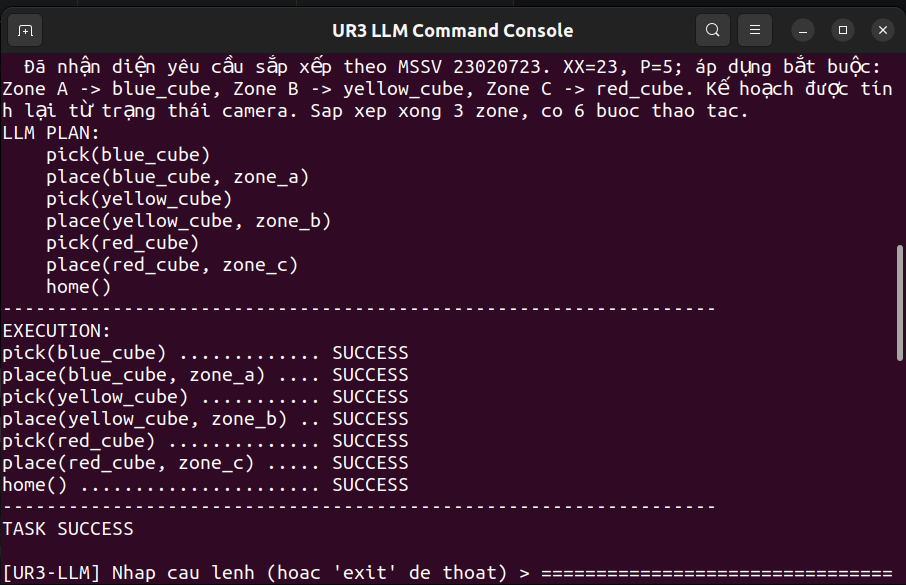
\includegraphics[width=0.82\textwidth]{images/mssv_success.png}
\caption{Kết quả sắp xếp MSSV: đúng ánh xạ P=5 và toàn bộ bước SUCCESS}
\label{fig:mssv-success}
\end{figure}

\subsection{Kịch bản 4 -- Zone bị chiếm, yêu cầu cốt lõi Bài 03}
Trong lần chạy minh họa, camera phát hiện \code{zone\_a} chứa
\code{red\_cube}; người dùng yêu cầu đặt \code{yellow\_cube} vào A. Kế hoạch
được sửa thành dời đỏ sang \code{zone\_temp\_3}, sau đó mới đặt vàng vào A.

\begin{figure}[H]
\centering
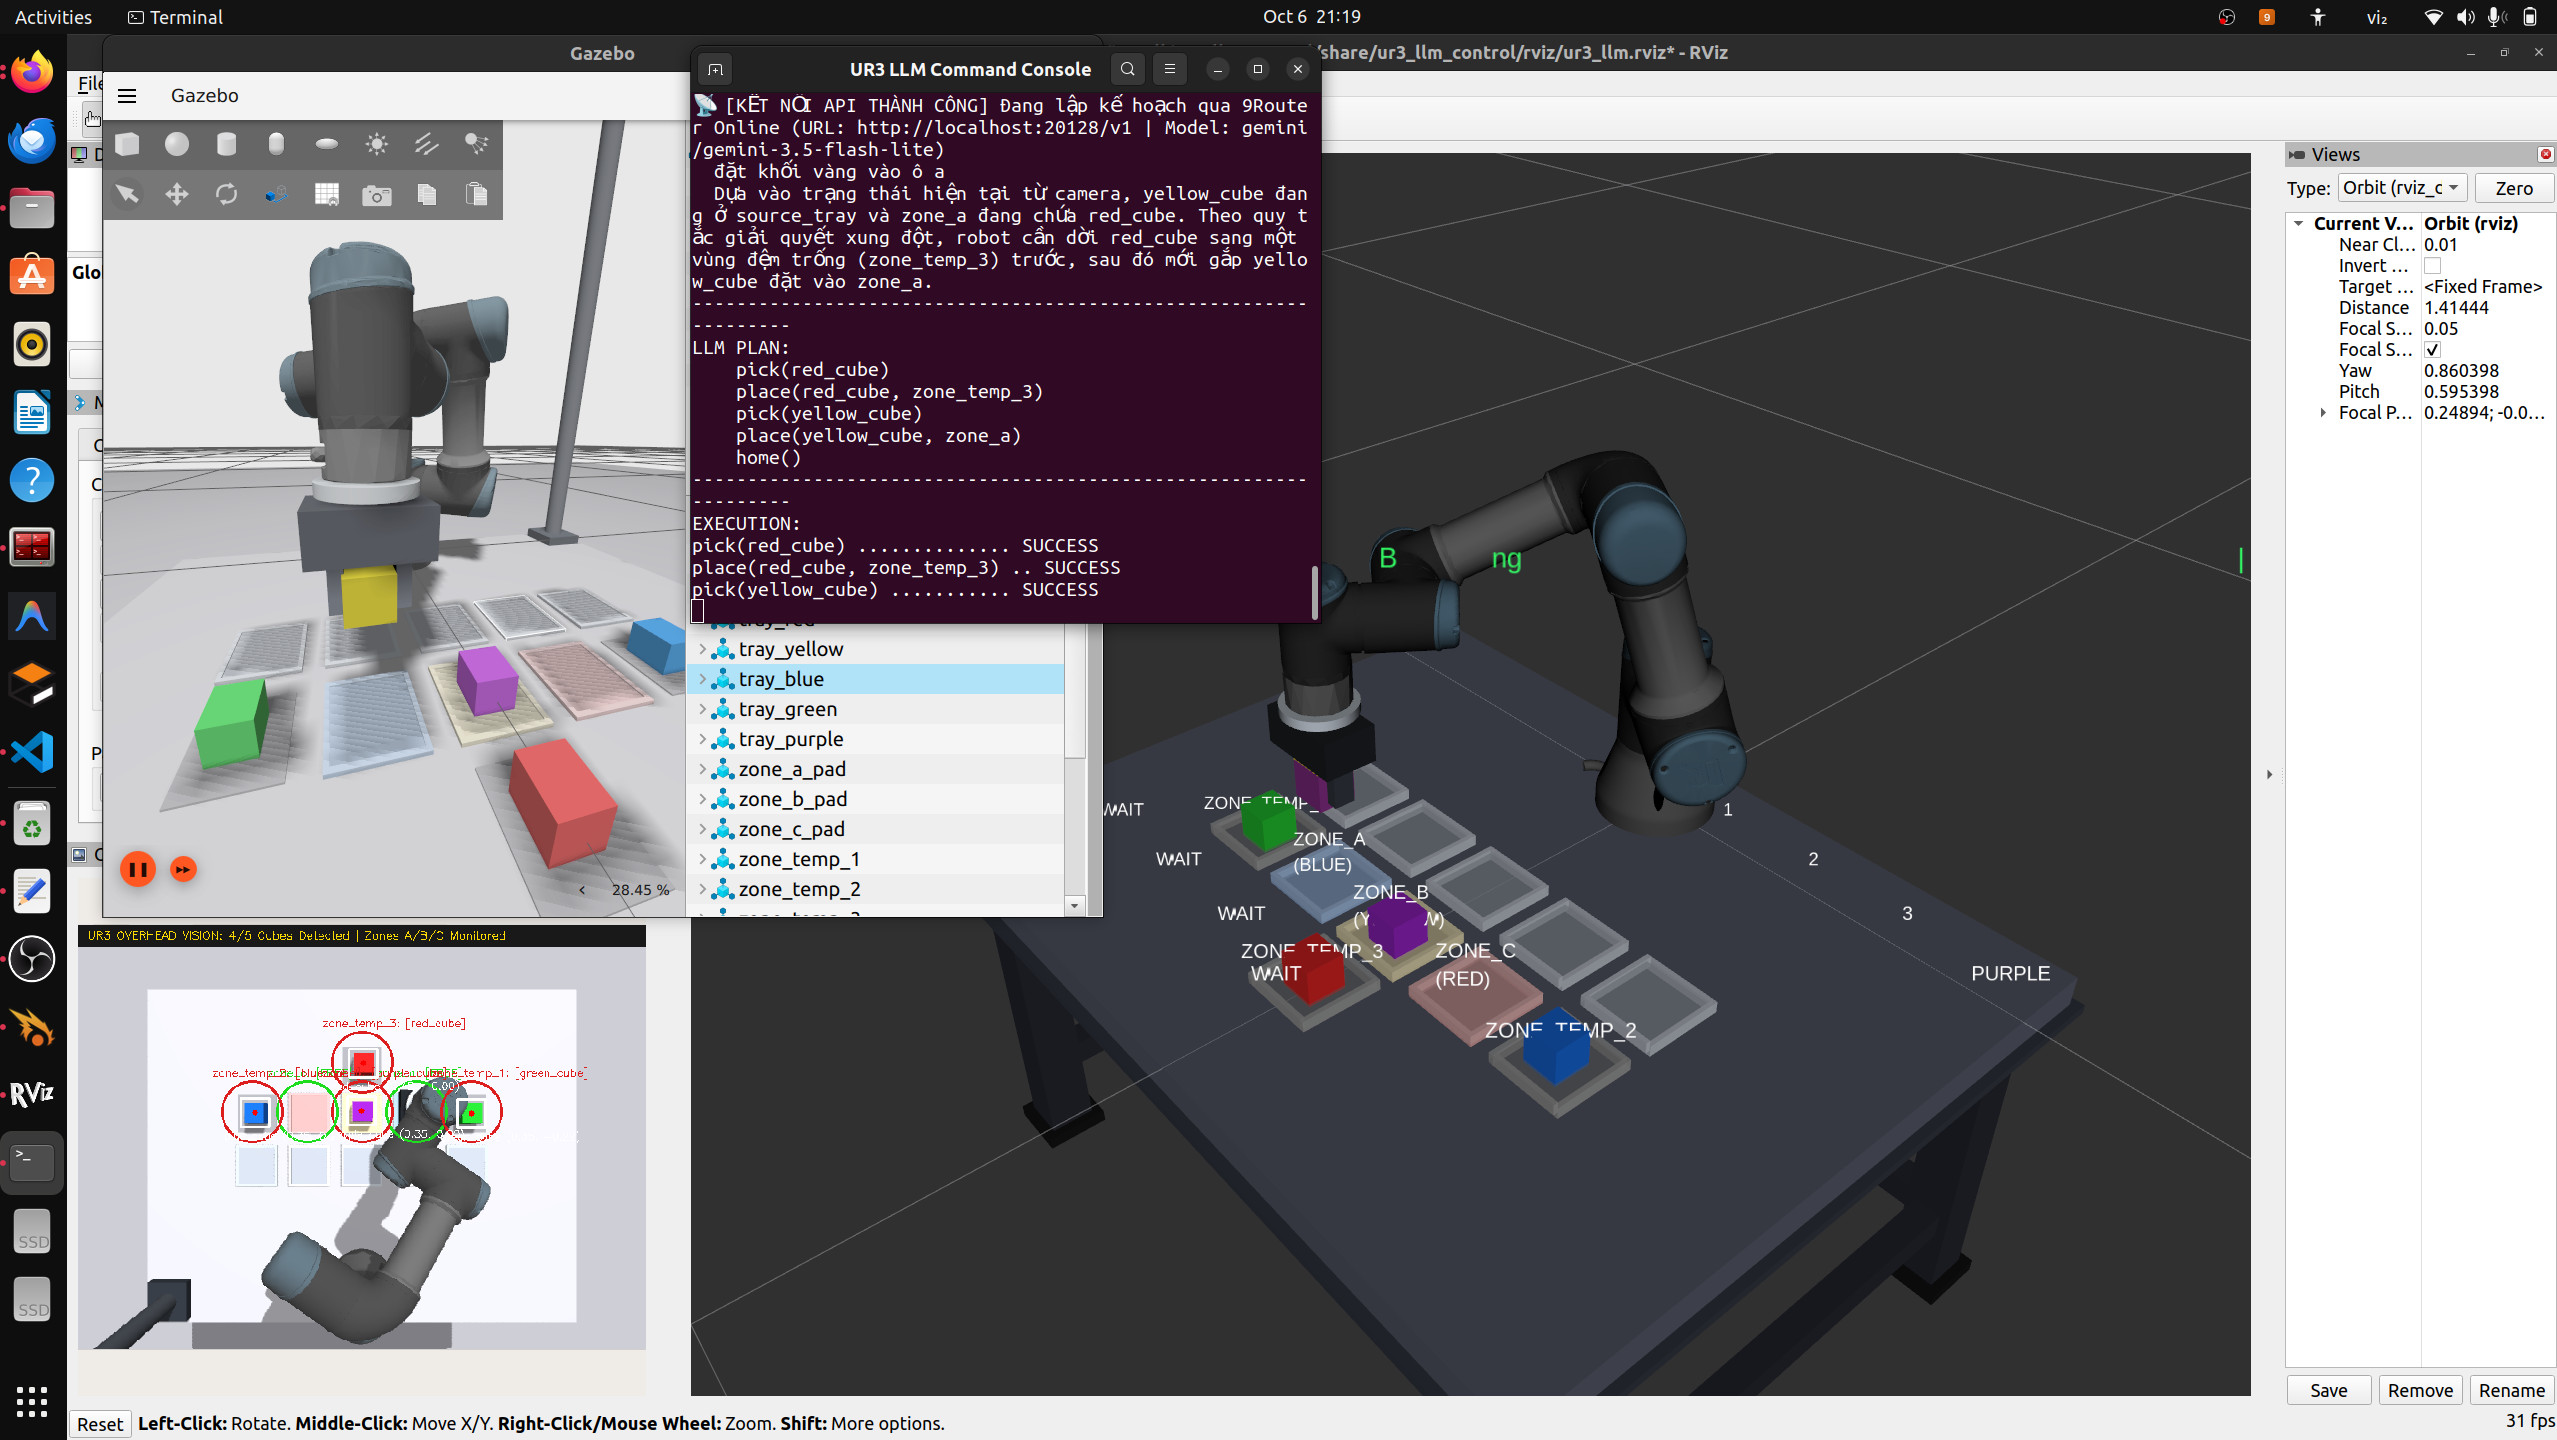
\includegraphics[width=0.98\textwidth]{images/conflict_execution.png}
\caption{Thực thi xung đột: dời red\_cube khỏi zone A rồi gắp yellow\_cube}
\label{fig:conflict-execution}
\end{figure}

Ảnh camera annotated ở góc trái dưới hiển thị vòng zone màu đỏ khi bị chiếm và
nhãn occupant. Gazebo cho thấy cube đang được kẹp vật lý; terminal ghi từng
bước \code{SUCCESS}. Sau khi hoàn tất, tay về home, \code{yellow\_cube} nằm ở A
và \code{red\_cube} nằm tại vùng tạm.

\begin{figure}[H]
\centering
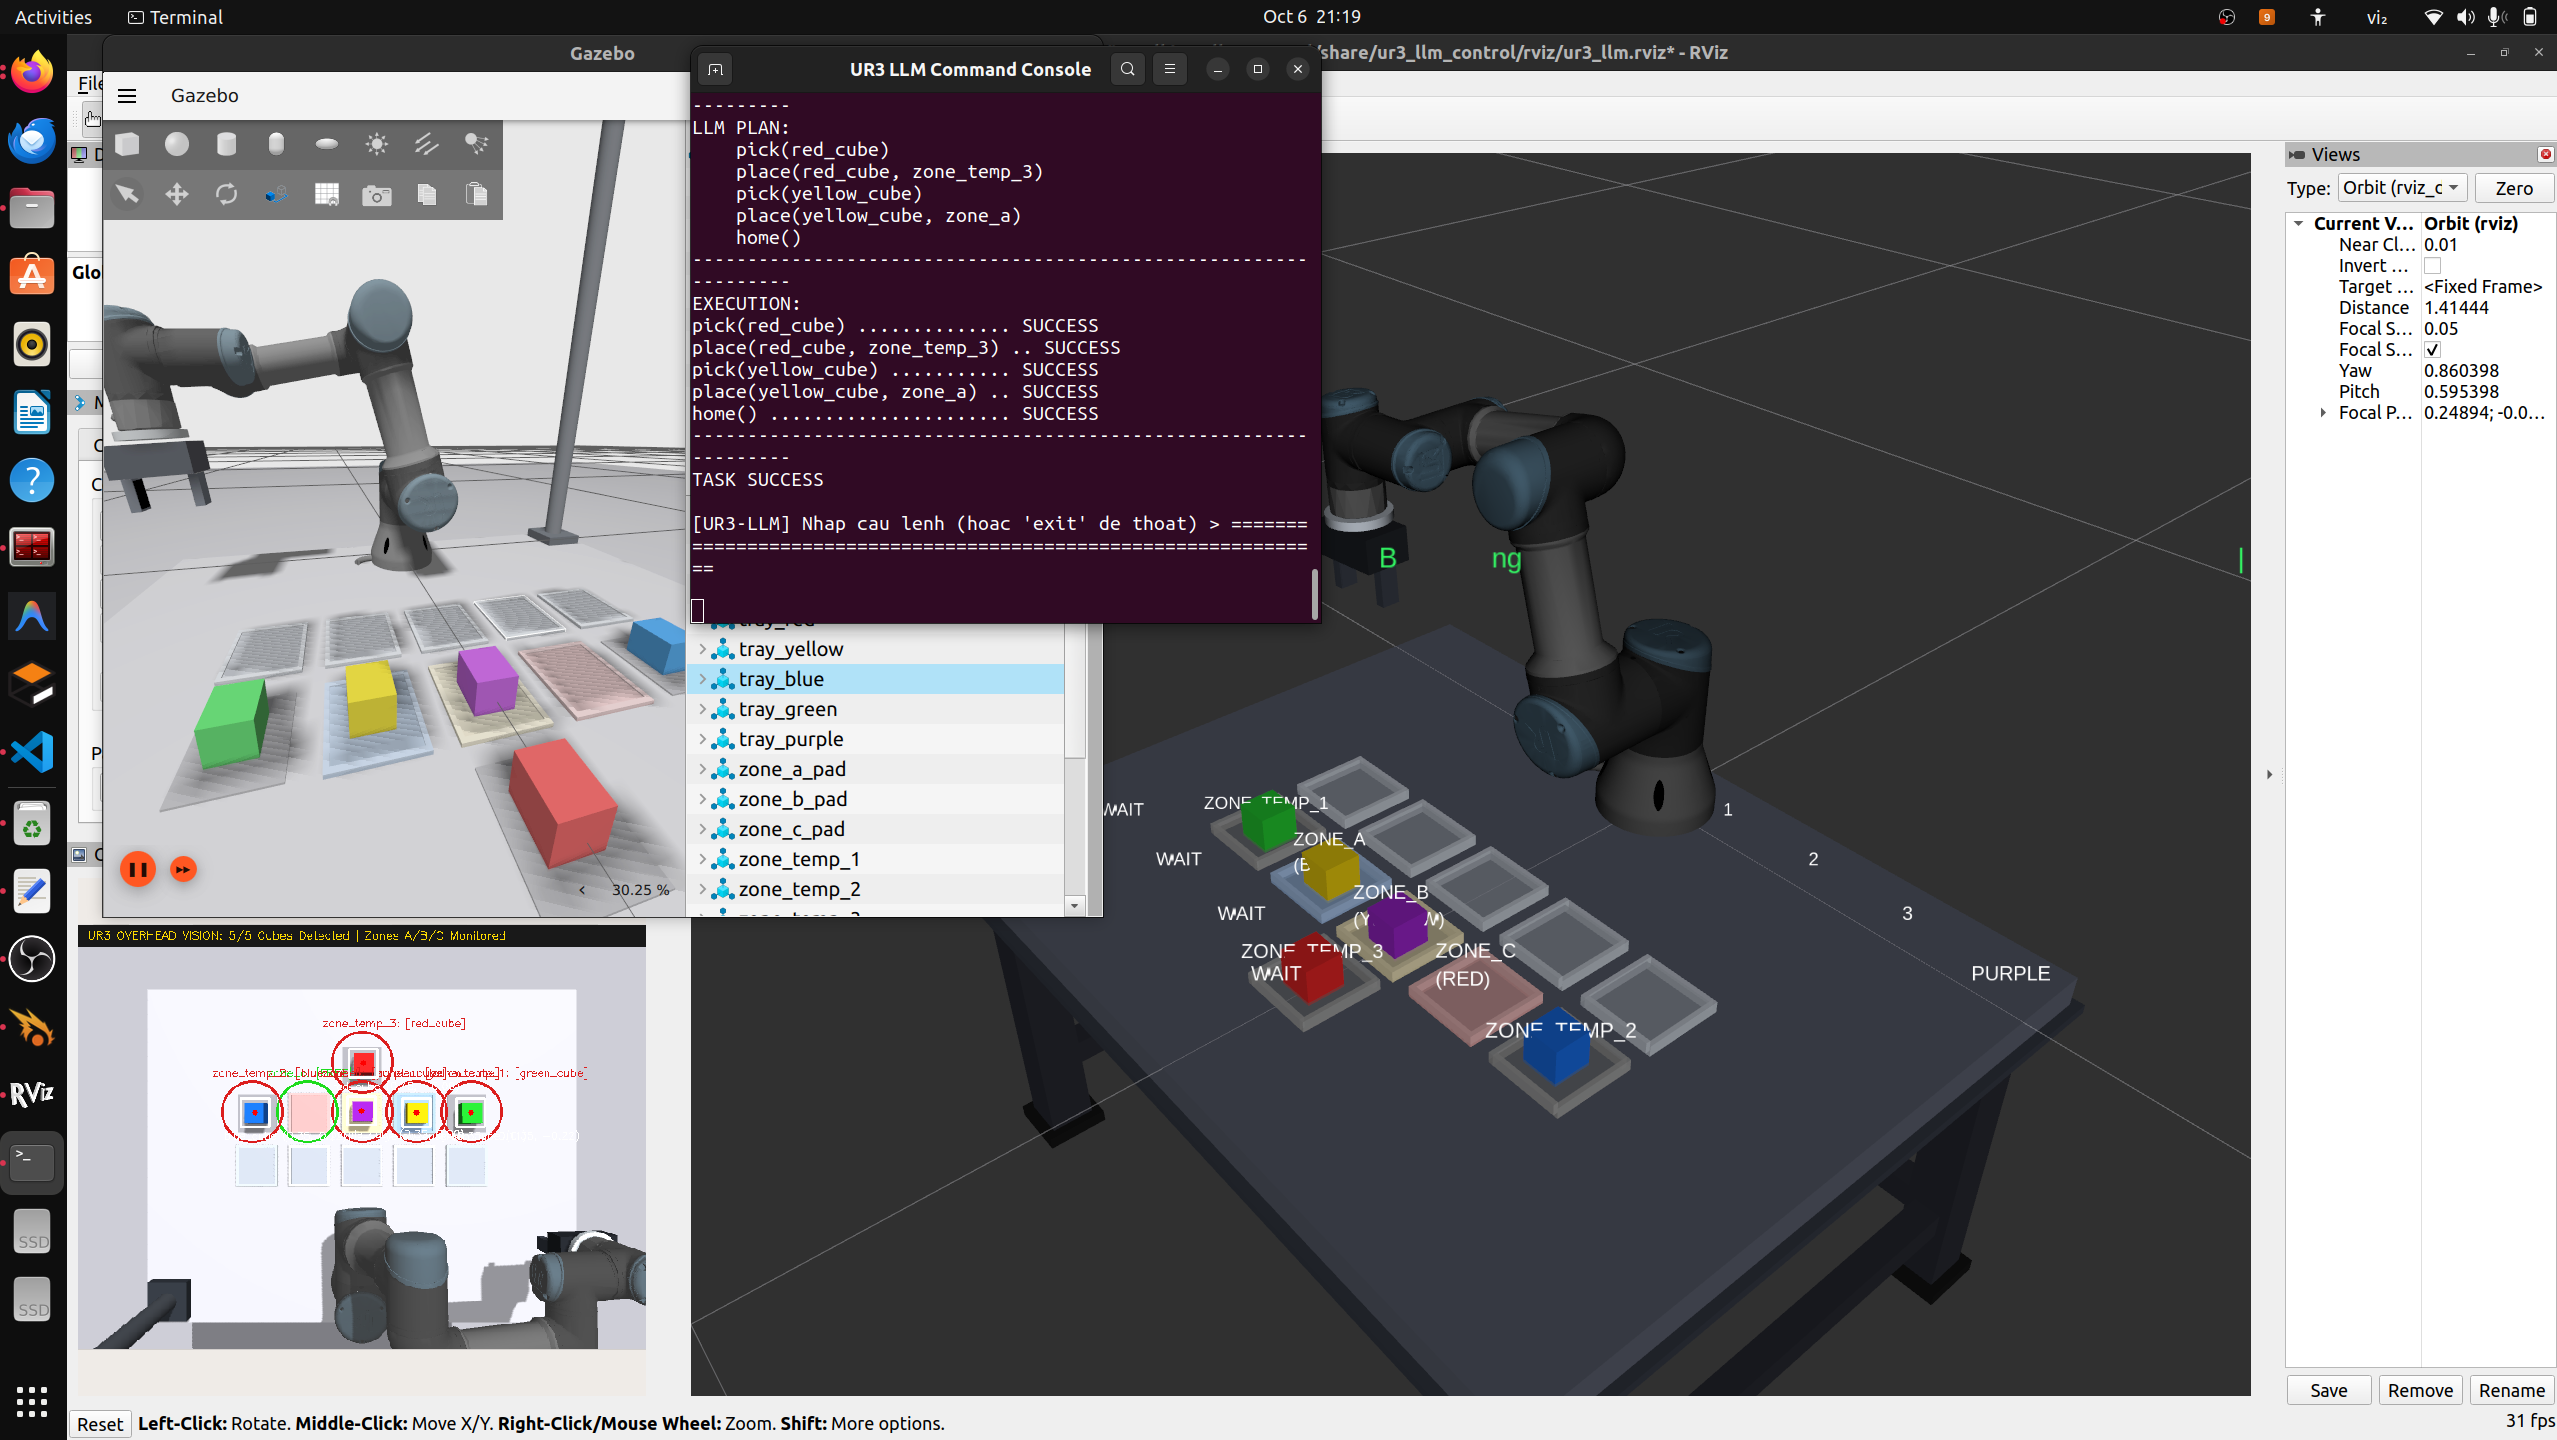
\includegraphics[width=0.98\textwidth]{images/conflict_success.png}
\caption{Kết quả kịch bản vùng bị chiếm: toàn bộ chuỗi báo TASK SUCCESS}
\label{fig:conflict-success}
\end{figure}

\subsection{Kịch bản 5 -- Hoán đổi hai khối}
\textbf{Lệnh:} \code{Hoán đổi vị trí khối đỏ và khối xanh lam.}

LLM chọn \skill{swap(red\_cube,blue\_cube)}. Validator kiểm tra hai object hợp
lệ và khác nhau. Skill chọn buffer trống, thực hiện ba chu kỳ pick/place như mô
tả ở mục trước. Kỳ vọng cuối: hai cube đổi vị trí chính xác, buffer trở lại trống
và gripper không còn giữ vật.

\subsection{Kịch bản 6 -- Xếp chồng và các skill quản trị}
Với lệnh \code{Stack the purple cube on top of the green cube}, robot gắp tím,
di chuyển trên xanh lá, hạ tới cao độ đặt bằng cao độ thông thường cộng 40 mm,
nhả rồi rút lên. \skill{inspect\_scene()} in trạng thái mà không di chuyển;
\skill{clear\_zone(zone\_c)} dời occupant ra vị trí trống;
\skill{reset\_scene()} trả từng cube về khay nguồn bằng pick/place vật lý.

\subsection{Kịch bản 7 -- Từ chối kế hoạch sai}
Các trường hợp object lạ, zone ngoài whitelist, place khi chưa pick, hai pick
liên tiếp, hoặc không còn buffer hợp lệ đều bị từ chối trước khi robot chạy.
Ví dụ \code{Move the apple to zone X} không thể vượt qua whitelist object và
zone. Đây là khác biệt quan trọng giữa văn bản do LLM tạo và lệnh robot được
phép thực thi.

\subsection{Kiểm thử phần mềm}
Bộ test \code{test\_plan\_safety.py} bao phủ:
\begin{itemize}
  \item dời vật cản trước khi gắp target;
  \item dùng zone đích trống khi các zone tạm đã đầy;
  \item từ chối an toàn khi không có buffer;
  \item toàn bộ 720 cách đặt năm cube vào sáu zone vật lý;
  \item giữ thứ tự khi người dùng yêu cầu trình tự;
  \item các biến thể câu lệnh MSSV tiếng Việt/Anh;
  \item thay kế hoạch MSSV sai do LLM online bằng ánh xạ chính xác;
  \item từ chối kế hoạch trộn sai màu.
\end{itemize}
Kết quả phiên bản báo cáo: \textbf{13/13 test passed}. Package cũng được kiểm
tra bằng \code{colcon build --packages-select ur3\_llm\_control
--symlink-install} và build thành công.

% =============================================================================
\section{Hướng dẫn cài đặt và chạy demo}

\subsection{Build package}
\begin{lstlisting}[language=bash,caption={Build workspace ROS 2}]
cd ~/ur3_ws
source /opt/ros/humble/setup.bash
colcon build --packages-select ur3_llm_control --symlink-install
source install/setup.bash
\end{lstlisting}

\subsection{Cấu hình LLM và launch}
Khóa API được truyền qua biến môi trường, không ghi vào repository:
\begin{lstlisting}[language=bash,caption={Khởi động 9Router và hệ thống robot}]
# Terminal 1
npx 9router

# Terminal 2
cd ~/ur3_ws
source /opt/ros/humble/setup.bash
source install/setup.bash
export NINE_ROUTER_API_KEY="<khoa-cua-ban>"
ros2 launch ur3_llm_control llm_robot.launch.py
\end{lstlisting}

Sau khi Gazebo, RViz và camera ổn định, nhập lệnh trong console. Có thể kiểm tra
trạng thái camera bằng:
\begin{lstlisting}[language=bash,caption={Kiểm tra scene state do camera công bố}]
ros2 topic echo --once /scene/camera_state
\end{lstlisting}
Trước một task mới, \code{camera\_active} phải là \code{true} và
\code{detected\_count} bằng 5. Đối với demo bắt buộc, có thể đặt một cube vào B,
chờ hoàn tất, rồi yêu cầu cube khác vào B để quan sát chuỗi giải phóng vùng.

\subsection{Mã nguồn}
Mã nguồn Bài thực hành 03 được lưu tại nhánh \code{assignments\_3}:
\begin{center}
\url{https://github.com/bangrbt/ur3_ws/tree/assignments_3}
\end{center}

% =============================================================================
\section{Đánh giá và kết luận}

Hệ thống đã đáp ứng các điểm chính của Bài 03: camera được dùng làm nguồn trạng
thái thay cho tọa độ khai báo cố định; gripper đóng/mở và tiếp xúc vật lý; vật
được giữ bằng joint chỉ sau khi hai ngón bao đúng cube; MoveIt 2 chịu trách nhiệm
IK, quỹ đạo và va chạm; LLM chỉ làm việc ở cấp skill. Cơ chế giải phóng vùng
đích cho phép xử lý tình huống không thể pick--place trực tiếp, còn các lớp
validator và camera verification ngăn báo thành công khi môi trường không đạt
hậu điều kiện.

Việc chia profile tốc độ theo giai đoạn, khóa hướng top-down, dùng Cartesian cho
đoạn thẳng đứng, hạn chế bước nhảy khớp và căn tâm theo contact giúp chuyển động
ngắn, mượt và ổn định hơn. Ánh xạ MSSV được tách khỏi tính ngẫu nhiên của LLM nên
luôn đúng A=xanh lam, B=vàng, C=đỏ ngay cả khi môi trường ban đầu có chu trình
chiếm chỗ.

Hướng phát triển tiếp theo là bổ sung visual servo bằng camera cổ tay cho sai số
cục bộ, dùng depth camera để ước lượng trực tiếp cao độ vật, và thay phân đoạn
màu bằng detector học sâu khi môi trường ánh sáng phức tạp. Các mở rộng này có
thể đặt phía dưới lớp skill hiện tại mà không trao quyền sinh lệnh khớp cho LLM.

\end{document}
